\chapter{Mandala-1}

\begin{figure}[htbp]
\begin{center}
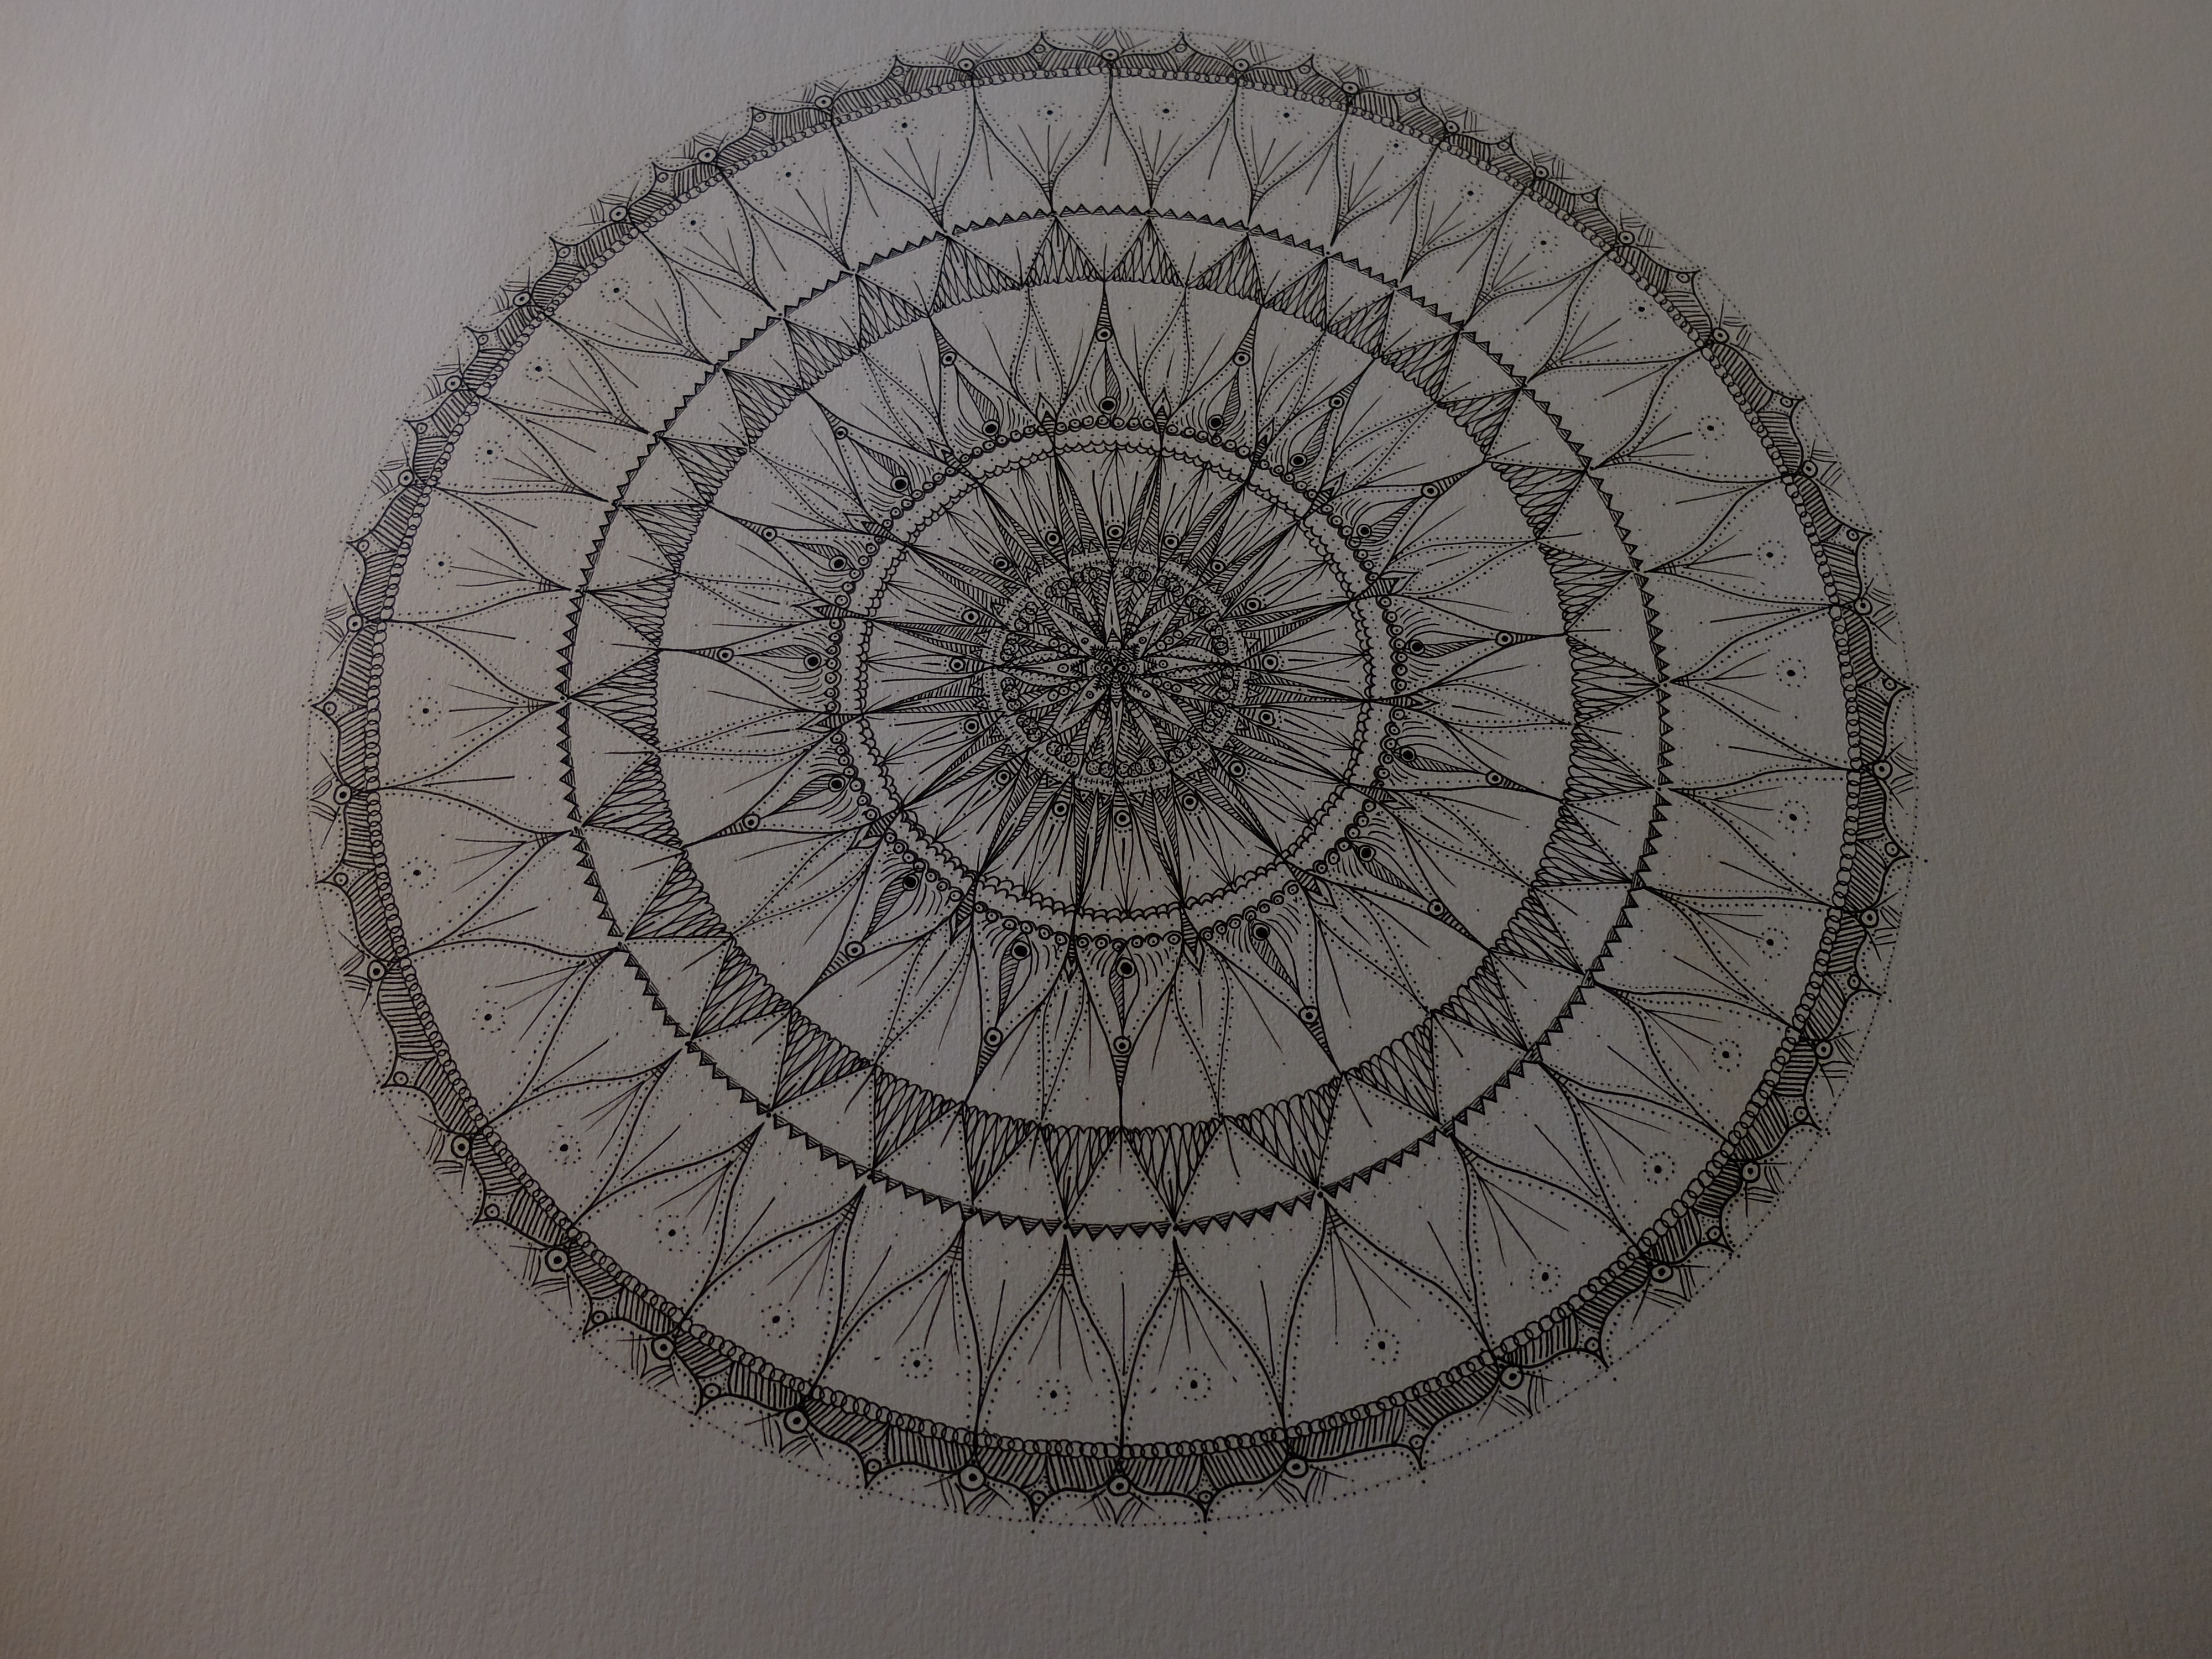
\includegraphics[scale=.05]{../eps/Final_Mandala_1.eps}
\label{label}
\end{center}
\end{figure}

\newpage
In the following 6 mandalas you will find a description of each mandala which states each states how long it took to produce, the process of making it, key words, any dialogue which may have been created as well as picture which illustrate the progression. 

I also want to highlight that I entered each mandala with my heart pouring onto the page. I gave myself permission to feel everything and I did not censor anything through creating the mandalas. I felt and sat inside all my emotions. My body was tight and sore all the time and I sensed the heaviness of my aches within my neck and muscles. Each stroke said a word. Each line escaped my fluttering of condensed grief. It felt as if every dot transported small pieces of my emotions on to the page. Every circle translated my inner self without words. I cried uncontrollably, but the tears lessened as my inquiry progressed and vanished by the end. I did not intend to write my thesis with such personal data, but every time I picked up a pen and drew inside a circle, I was transported to unpack myself and work through what was coming to the surface deep within. I felt I was held and safe inside the walls of a circle. The repetitious and circular motion calmed me even though I was expressing anger, fear and negativity. Thus, I happily sunk into the depths of my despair and the unknown of what the future holds for me. 

My first mandala took me 9 sittings to complete. I started with 20 minutes, 50 minutes, 25 minutes, 20 minutes, 1.15 minutes, 15 minutes, 5 minutes, 50 minutes, and 35 minutes. As I drew I stopped at different stages and wrote what I was feeling, thinking, sensing and imagining. I started from the middle and just drew with no intention. The process was purely intuitive and emergent. 

\Date: Finished on the 24th of May 2015.
\Total: 3 hours of drawing
%Mandala 1
I tracked my thoughts, feelings, memories & sensations within the process of creating a mandala, I wrote the following:


\begin{table}[htp]
\caption{default}
\begin{center}
\begin{tabular}{|c|c|}
I see hand saws on the left and right (in the inside circles)
In the middle looks like people with lots of hands and feet
Also looks like fish 
My lower back is sore
I like these new pens I bought
I'm hungry
Outside is a beautiful blue sky, but really cold 
I see spirals, lines, dots
I drew a circle, does not feel right
Draw little circles over larger circles mmm, that's better
I need to overlap my life with friends and family
I crunch my right elbow
I smile
I put relaxing music on
^ shape
Opening
Many people in the crowd
Triangles
Eyes, worried eyes
Going left is easy, going right is hard (Drawing left and right)
I wonder is it the same when I ride my bike and turn left and right? I can not remember but there is definitely one direction when turning which seems more difficult for me. 
It feels weird drawing from right to left, normally I go from left to right
I notice that I repeat what I am thinking
I want someone that is optimistic 
Why did I stay with him, if he could never really commit to me and love me without the fear that was weighing him down?
Stay in the moment and be present in the moment Rachel 
I felt I would grow old with him, but I guess he did not have the same mentality
I want someone who is optimistic, not pessimistic
Drawing a petal, I think he loves me, he loves me not, he loves me, he loves me not, I laugh
Change pen to the bigger size
1234
Circle, dots, third eye, native American Indian
Outer dots on the edge, line, dots with purpose and conviction
Become alive again
Go for a run, getting hungry
Went for run, but after 10 minutes I seemed to pull my right Achilles tendon/calf muscle, or did I get a huge cramp? I can not figure it out
In the drawing I feel I made a mistake, but I turn it to make it look and feel better
Eyes, eyes, eyes, repeated 
Eye balls
Bumble bee
Gate, snake
Lower back pain
Sorry I miss you already (listening to Pearl Jam)
Snake, going out
Shuffle songs I wish you stayed (I anticipated when you would come home), Ha, Ho lets go, Life wasted
Half petal, one sided?
Evolution
Thought What do I want? What is important to me? 
My next relationship, what are my needs! Ha, Ho, lets go
Dots
Searching for answers
Feathers
Lost in songs
Plant 
Right shoulder blades and neck are really tight
rock in the free world
I am thirsty
Stayed up late
I am open to new possibility, opportunities
Surround myself with inspiring people 
Bond, link circles
Getting lost in the dots
Circles- think of the bond, connection with each other 
My desire for a connection and a bond again with a partner
Oh that was a short line
Thought Where have I fell short in my life?
Wish him all the best!
Still feel that one day he will come and say what was not said
Would I want him back anyway?
His actions speak louder than words and its obvious he does not want me back
Anyway.. Im tired, I remember the conversations that I have had, Flower, Elbow is sore 
\end{tabular}
\end{center}
\label{default}
\end{table}%

 
I clustered the main words in groups which I felt related to each other and then titled each one:
\begin{enumerate}
\item Tired; Sore, tight, fell short, worried, snake, snake, tired
\item Why; I felt
\item Grow; Hungry, thirsty, see, grow
\item Connection; Bond, link, conversations, become alive again, connection
\item Open; Optimistic, obvious, possibilities, opening, open
\item Action; Flower, gate, action 
\end{enumerate}

The development of making mandala 1:

%FIGURE 2-MANDALA 1-STARTING OFF WITHIN THE CENTRE

%FIGURE 3- GROWING OUTWARDS

%FIGURE 4- STEMMING OUT

%FIGURE 5-ADDING MORE DETAIL

%FIGURE 6-STARTING TO BUILD

%FIGURE 7- KEEPS GROWING

%FIGURE 8-ALMOST THERE


%FIGURE 9-FINAL MANDALA 1



